% Copyright (c) 2012 by Michał Nazarewicz <mina86@mina86.com>
% Distributed under the terms of the Creative Commons
% Attribution-ShareAlike 3.0 Unported (CC BY-SA 3.0) license.
\documentclass{beamer}
\usepackage[utf8]{inputenc}
\usepackage[T1]{fontenc}
\usepackage{lmodern}
\usepackage[polish]{babel}
\usepackage{pgf}
\usepackage{units}
\usepackage{lmodern}
\usepackage{color}
\usepackage{listings}
\usepackage{amsmath}
\usepackage[super]{nth}

\newcommand{\notimplies}{%
  \mathrel{{\ooalign{\hidewidth$\not\phantom{=}$\hidewidth\cr$\implies$}}}}

\definecolor{gray}{RGB}{102,102,102}
\definecolor{darkgreen}{RGB}{0,128,0}

\lstset{
  language=C,
  basicstyle=\small\rmfamily,
  numbers=left,
  numberstyle=\tiny\color{gray},
  stepnumber=1,
  numbersep=5pt,
  showspaces=false,
  showstringspaces=false,
  showtabs=false,
  tabsize=8,
  captionpos=b,
  breaklines=true,
  breakautoindent,
  columns=fullflexible,
  morekeywords={inline,bool},
  keywordstyle=\color{blue}\bfseries,
  commentstyle=\color{darkgreen}\itshape,
  stringstyle=\color{red}\ttfamily
}
\lstdefinelanguage{diff}{
  morecomment=[f][\color{blue}]{@@},     % group identifier
  morecomment=[f][\color{red}]-,         % deleted lines
  morecomment=[f][\color{darkgreen}]+,   % added lines
  morecomment=[f][\color{gray}]{---},    % Diff header lines (must appear after +,-)
  morecomment=[f][\color{gray}]{+++},
}
\def\code{\lstinline[basicstyle=\rmfamily]}

\usetheme{Frankfurt}

% Shrink the margins slightly.
\setbeamersize{text margin left=5mm}
\setbeamersize{text margin right=5mm}

% Remove navigation symbols. They are never used anyway.
\setbeamertemplate{navigation symbols}{}

% Make more room on notes pages (when used).
\setbeamertemplate{note page}[plain]
\setbeamerfont{note page}{size=\scriptsize}

% gray footnotes, no rule.
% FIXME: This is broken. The gray continues onto subsequent slides.
% Note: footnotes are generally a bad idea in presentations.
\setbeamercolor{footnote mark}{fg=gray}
\renewcommand{\footnoterule}{}

\setbeamertemplate{footline}{}

\newcommand\Section[1]{%
\section{#1}%
\begin{frame}%
\frametitle{Zarys prezentacji}
\tableofcontents[currentsection]%,sections=\thesection]%
\end{frame}}


\newcommand\theauthor{Michał Nazarewicz}
\newcommand\theemail{mina86@mina86.com}
\title{Continuous Memory Allocator}
\subtitle{Alokacja dużych obszarów ciągłej fizycznie pamięci}
\author[\theauthor]{%
  \texorpdfstring{\theauthor\vskip 8pt%
    \scriptsize\href{mailto:\theemail}{\theemail}}{%
    \theauthor}}
\institute{Instytut Informatyki Politechniki Warszawskiej}
\date{\today}

\setbeamerfont{institute}{size={\fontsize{10pt}{12pt}}}
\setbeamerfont{date}{size={\fontsize{8pt}{10pt}}}


\begin{document}

\begin{frame}
  \titlepage
\end{frame}

\begin{frame}
  \frametitle{Zarys prezentacji}
  \tableofcontents
\end{frame}

\Section{Wstęp}
\subsection{Why physically contiguous memory is needed}

\begin{frame}
  \frametitle{The mighty MMU}

  \begin{itemize}
  \item Modern CPUs have MMU.
    \begin{itemize}
    \item Virtual $\rightarrow$ physical address.
    \end{itemize}
  \item Virtually contiguous $\notimplies$ physically contiguous.
  \item So why bother?
  \end{itemize}
\end{frame}

\begin{frame}
  \frametitle{System devices}

  \begin{itemize}
  \item MMU stands behind CPU.
  \item There are other chips in the system.
  \item Some require large buffers.
    \begin{itemize}
    \item 5-megapixel camera anyone?
    \end{itemize}
  \item On embedded, there's plenty of those.
  \end{itemize}
\end{frame}

\begin{frame}
  \frametitle{The mighty DMA}

  \begin{itemize}
  \item DMA can do vectored I/O.
  \item Gathering buffer from scattered parts.
  \item Contiguous for the device $\notimplies$ physically contiguous.
  \item So why bother?
  \end{itemize}
\end{frame}

\begin{frame}
  \frametitle{The mighty system MMU}

  \begin{itemize}
  \item What about a~system MMU?
    \begin{itemize}
    \item Address coming from the device $\rightarrow$ physical
      address
    \end{itemize}
  \item Same deal as with CPU's MMU.
  \item So why bother?
  \end{itemize}
\end{frame}

\begin{frame}
  \frametitle{Cost, speed \& power}

  \begin{itemize}
  \item Every chip costs.
    \begin{itemize}
    \item Money and power.
    \end{itemize}
  \item More complex chips cost more.
  \item Not all systems have DMA with SG or system MMU.
  \item System MMU takes time.
  \end{itemize}
\end{frame}

% Copyright (c) 2012 by Michał Nazarewicz <mina86@mina86.com>
% Distributed under the terms of the Creative Commons
% Attribution-ShareAlike 3.0 Unported (CC BY-SA 3.0) license.

\subsection{Solutions to the problem}

\begin{frame}
  \frametitle{Lie to the kernel}

  \begin{itemize}
  \item Lie to the kernel about amount of memory.
    \begin{itemize}
    \item Easily done with a~\code{mem} parameter.
    \item Kernel won't touch memory hidden via \code{mem}.
    \end{itemize}
  \item Assign buffers to each device that might need it.
  \item Platform dependent.
  \item Requires fiddling with boot loader.
  \item \ldots
  \end{itemize}
\end{frame}

\begin{frame}
  \frametitle{Reserve and assign at boot time}

  \begin{itemize}
  \item Reserve memory during system boot time.
  \item Assign buffers to each device that might need it.
  \item Less platform dependent.
  \item Boot loader is left alone.
  \item While device is not being used, memory is wasted.
  \end{itemize}
\end{frame}

\begin{frame}
  \frametitle{Reserve but allocate on demand}

  \begin{itemize}
  \item Reserve memory during system boot time.
  \item Provide API for allocating from that reserved pool.
  \item Less memory is reserved.
  \item But it's still wasted.
  \end{itemize}

  \begin{itemize}
  \item bigphysarea
  \item Physical Memory Manager
  \end{itemize}
\end{frame}

\begin{frame}
  \frametitle{Reserve but give back}

  \begin{itemize}
  \item Reserve memory during system boot time.
  \item Give it back
    \begin{itemize}
    \item but set it up so only movable pages can be allocated.
    \end{itemize}
  \item Provide API for allocating from that reserved pool.
  \item Migrate pages on allocation.
  \end{itemize}

  \begin{itemize}
  \item Contiguous Memory Allocator
  \end{itemize}
\end{frame}

\Section{Pamięć w Linuksie}
% Copyright (c) 2012 by Michał Nazarewicz <mina86@mina86.com>
% Distributed under the terms of the Creative Commons
% Attribution-ShareAlike 3.0 Unported (CC BY-SA 3.0) license.

\subsection{Przegląd alokatorów}

\begin{frame}
  \frametitle{Alokatory pamięci Linuksa}

  \begin{center}
    \includegraphics[width=\textwidth]{build/linux-allocators--base.eps}
  \end{center}
\end{frame}

\begin{frame}
  \frametitle{\code{kmalloc}, \code{vmalloc} itp.}

  \begin{itemize}
  \item \code{kmalloc}
    \begin{itemize}
    \item Najczęściej stosowany alokator.
    \item Ciągłe fizycznie obszary $\le$
      \unit[4]{MiB}\textcolor{gray}{$^\dagger$}.
    \item Koszysta z~alokatora stron.
    \end{itemize}

  \item \code{vmalloc}
    \begin{itemize}
    \item Alokacje nieciągłe fizycznie.
    \item Koszysta z~alokatora stron.
    \end{itemize}

  \item \code{kmem_cache}
    \begin{itemize}
    \item Alokacja obszarów o~z~góry zadanym rozmiarze.
    \item Inny interfejs dla kmalloc().
    \end{itemize}

  \item \code{mempool}
    \begin{itemize}
    \item Interfejs do tworzenia podręcznych pul buforów.
    \item Zazwyczaj korzysta z~kmem\_cache i~kmalloc().
    \end{itemize}
  \end{itemize}
\end{frame}

\begin{frame}
  \frametitle{Alokator czasu startu systemu}

  \begin{itemize}
  \item Memblock jest aktywny przy starcie systemu.
  \item Przechowuje listę dostępnych obszarów pamięci RAM.
  \item Prosty interfejs do alokowania buforów.
  \item Możliwe jest rezerwowanie dużych bloków.
  \item Pozostała wolna pamięć jest przekazywana do alokatora stron.
  \end{itemize}
\end{frame}

\begin{frame}
  \frametitle{Alokator przeznaczony dla urządzeń}

  \begin{itemize}
  \item DMA API umożliwia alokowanie buforów DMA.
  \item Są one dostępne dla urządzeń na płycie głównej.
    \begin{itemize}
    \item W~szczególności dla kontrolera DMA.
    \end{itemize}
  \item Implementacja zależna od architektury.
  \item Często korzysta z~alokatora stron.
  \end{itemize}
\end{frame}

\begin{frame}
  \frametitle{Alokatory pamięci Linuksa, II}

  \begin{center}
   \includegraphics[width=\textwidth]{build/linux-allocators--important.eps}
  \end{center}
\end{frame}

\subsection{Page allocator}

\begin{frame}[fragile]
  \frametitle{Pages and page blocks}

  \begin{itemize}
  \item Linux manages memory in units of pages.
    \begin{itemize}
    \item Typically \unit[4]{KiB} in size.
    \end{itemize}
  \item Page can have order ranging from 0 to 10.\footnote{Strictly
    speaking, from zero to one less than \code{MAX_ORDER} which is
    usually 11.}
    \begin{itemize}
    \item $n$-order page consists of $2^n$ \unit[4]{KiB} pages.
    \item 10-order page is called max-order page.
    \end{itemize}
  \item Pages are grouped into page blocks.
  \item Page block consists of 1024 pages, same size as max-order
    page.\footnote{This actually depends, but it's the case for ARM
      and x86.}
  \item {\footnotesize Let's forget about zones or NUMA.}
  \end{itemize}
\end{frame}

\begin{frame}
  \frametitle{Pages and page blocks, cont}
  \begin{center}
  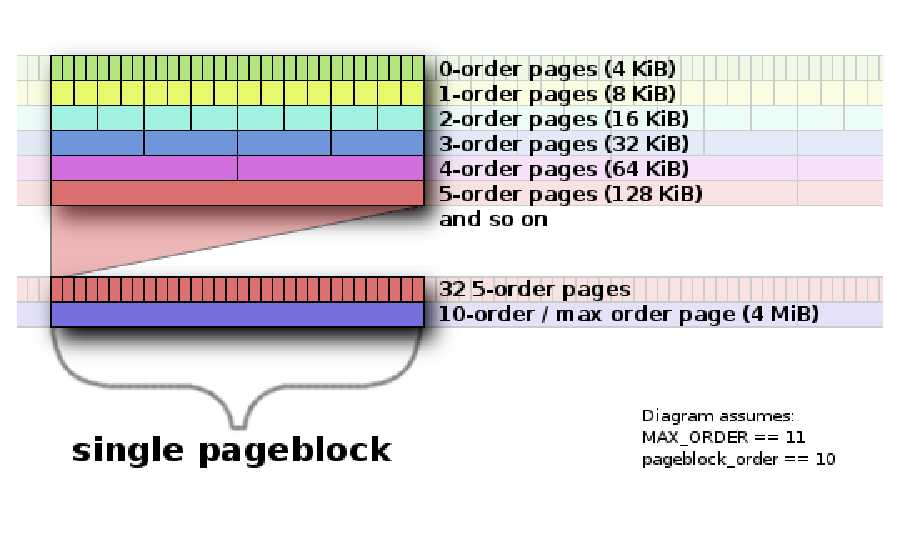
\includegraphics[width=0.9\textwidth]{build/pages.eps}
  \end{center}
\end{frame}

\begin{frame}
  \frametitle{Buddy allocator}
  \begin{columns}[c]

    \column{0.6\textwidth}
    \begin{itemize}
    \item Page allocator uses buddy allocation algorithm.
      \begin{itemize}
      \item Hence different names: buddy system or buddy allocator.
      \end{itemize}
    \item Allocations are done in terms of orders.
    \item User can request order from 0 to 10.
    \item If best matching page is too large, it's recursively split
      in half (into two buddies).
    \item When releasing, page is merged with its buddy (if free).
    \end{itemize}

    \column{0.4\textwidth}
    \begin{center}
    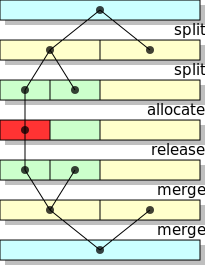
\includegraphics[width=0.9\textwidth]{build/alloc-free-cycle.eps}
    \end{center}
  \end{columns}
\end{frame}

\begin{frame}[fragile]
  \frametitle{Other allocators}

  \begin{itemize}
  \item Page allocator is used for allocations of $2^n$ pages.
  \item For more granular allocations other mechanisms are provided as
    well:
    \begin{itemize}
    \item \code{kmalloc()},
    \item \code{vmalloc()},
    \item Memory pools.
    \end{itemize}
  \item They fall outside of the scope of this presentation.
  \end{itemize}
\end{frame}

\begin{frame}[fragile]
  \frametitle{Migrate types}

  \begin{itemize}
  \item On allocation, user requests an unmovable, a~reclaimable or
    a~movable page.
    \begin{itemize}
    \item For our purposes, we treat reclaimable as unmovable.
    \end{itemize}
  \item To try keep pages of the same type together, each free page
    and each page block has a~migrate type assigned.
    \begin{itemize}
    \item But allocator will use fallback types.
    \item And migrate type of a~free page and page blocks can change.
    \end{itemize}
  \item When released, page takes migrate type of pageblock it belongs
    to.
  \end{itemize}
\end{frame}

\Section{Implementacja}
\subsection{Page allocator}

\begin{frame}[fragile]
  \frametitle{Pages and page blocks}

  \begin{itemize}
  \item Linux manages memory in units of pages.
    \begin{itemize}
    \item Typically \unit[4]{KiB} in size.
    \end{itemize}
  \item Page can have order ranging from 0 to 10.\footnote{Strictly
    speaking, from zero to one less than \lstinline|MAX_ORDER| which is
    usually 11.}
    \begin{itemize}
    \item $n$-order page consists of $2^n$ \unit[4]{KiB} pages.
    \item 10-order page is called max-order page.
    \end{itemize}
  \item Pages are grouped into page blocks.
  \item Page block consists of 1024 pages, same size as max-order
    page.\footnote{This actually depends, but it's the case for ARM
      and x86.}
  \item {\footnotesize Let's forget about zones or NUMA.}
  \end{itemize}
\end{frame}

\begin{frame}
  \frametitle{Pages and page blocks, cont}
  \begin{center}
  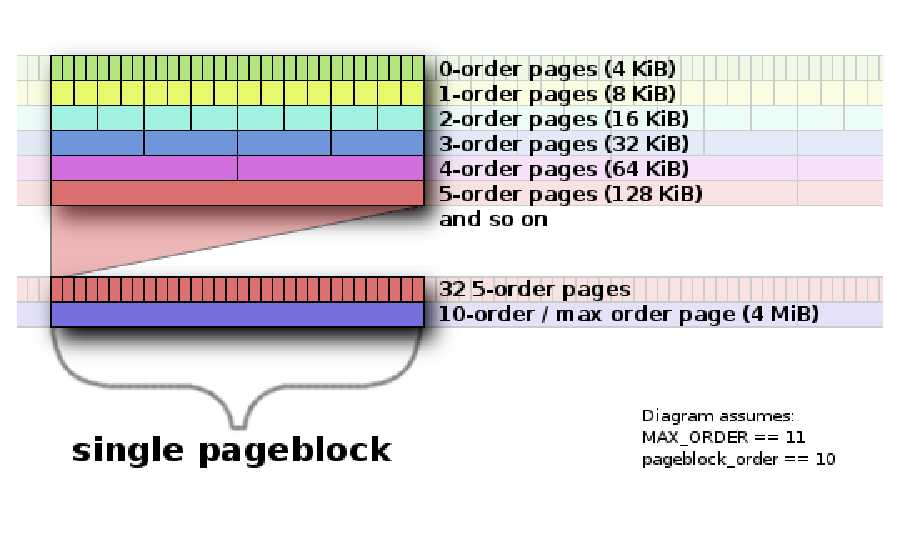
\includegraphics[width=0.9\textwidth]{build/pages.eps}
  \end{center}
\end{frame}

\begin{frame}
  \frametitle{Buddy allocator}
  \begin{columns}[c]

    \column{0.6\textwidth}
    \begin{itemize}
    \item Page allocator uses buddy allocation algorithm.
      \begin{itemize}
      \item Hence different names: buddy system or buddy allocator.
      \end{itemize}
    \item Allocations are done in terms of orders.
    \item User can request order from 0 to 10.
    \item If best matching page is too large, it's recursively split
      in half (into two buddies).
    \item When releasing, page is merged with buddy (if free).
    \end{itemize}

    \column{0.4\textwidth}
    \begin{center}
    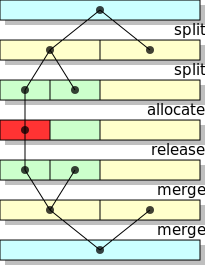
\includegraphics[width=0.9\textwidth]{build/alloc-free-cycle.eps}
    \end{center}
  \end{columns}
\end{frame}

\begin{frame}[fragile]
  \frametitle{Migrate types}

  \begin{itemize}
  \item On allocation, user requests an unmovable, a~reclaimable or
    a~movable page.
    \begin{itemize}
    \item For our purposes, we treat reclaimable as unmovable.
    \end{itemize}
  \item Movable pages will be set up so that they can be migrated.
  \end{itemize}

  \begin{itemize}
  \item To try keep pages of the same type together, each free page
    and each page block has a~migrate type assigned.
  \item But allocator will use fallback types.
  \item And migrate type of a~free page and page blocks can change.
  \end{itemize}
\end{frame}

% Copyright (c) 2012 by Michał Nazarewicz <mina86@mina86.com>
% Distributed under the terms of the Creative Commons
% Attribution-ShareAlike 3.0 Unported (CC BY-SA 3.0) license.

\subsection{CMA problems and future work}

\begin{frame}
  \frametitle{Problems}

  \begin{itemize}
  \item \code{get_user_pages()} makes migration impossible.
  \item ext4 does not support migration of journal pages.
  \item Some filesystems are not good on migration.
  \end{itemize}
\end{frame}

\begin{frame}
  \frametitle{Future work}
  \begin{itemize}
  \item Only swap.
  \item \href{http://lwn.net/Articles/340080/}{Transcendent memory}.
  \item \href{http://lwn.net/Articles/468896/}{\code{POSIX_FADV_VOLATILE}}.
  \end{itemize}
\end{frame}


\appendix

\section*{Pytania?}
\begin{frame}
  \begin{center}
    \vskip 2em
    {\Huge Dziękuję!}
    \vskip 2em
    
\includegraphics[width=0.3\textwidth]{build/interrogation.eps}
  \end{center}

  \vskip 2em

  \begin{itemize}
  \item \theauthor
  \item \href{mailto:\theemail}{\theemail}, \href{mailto:mpn@google.com}{mpn@google.com}
  \item \url{http://mina86.com/cma/}
  \end{itemize}

  \vskip 1em
  \hfill \href{http://creativecommons.org/licenses/by-sa/3.0}{%
    \includegraphics[height=0.8em,clip=true]{build/cc-by-sa.eps}}
\end{frame}

\end{document}
